\chapter {Further work}

\section{Size-based model}

\subsection{Background}

Phytoplankton organisms are significantly limited by nutrient diffusion and by sinking. These two crucial processes in water pose important constraints on phytoplankton morphological traits such as cell size. Cell size is therefore subject to an important selection pressure that tends to favour those shapes and sizes that allow phytoplankton access nutrient resources more efficiently while maintaining themselves in the surface waters to access light \citep{Litchman2008}. Size plays also a major role in growth and metabolism \citep{Finkel2009a}. The importance of this trait has motivated the development of a number of size-based ecological models. For example, \citet{Baird2007} developed a 1D, size-based model of three major group of organisms (phytoplankton, protozoan and metazoan) that takes into account a certain number of size-classes. Each of these classes of organisms could be further subdivided into defined functional groups or species that can be mathematically represented with state variables. Baird and Suthers' (\citeyear{Baird2007}) model is formulated independently of the number of size classes, this help to reduce the complexity in terms of number of state variables and free parameters. However, with increasing number of size classes the model becomes computationally more expensive without any apparent benefit in the understanding of the system dynamics and with a clear increase in model sensitivity. Although size-based, which is still an unusual practice in phytoplankton modelling, this approach follows the typical tendency of introducing extra complexity in models, beyond the simple nutrient-phytoplankton-zooplankton-detritus (NPZD) configurations, when more size classes are considered. This tendency, however, faces numerous difficulties, particularly because of the poorly understood ecology, the lack of data, the problems connected with aggregating diversity within functional groups into meaningful state variables and constants, and the higher sensitivity of outputs to the parameterizations in question \citep{Anderson2005}.

Interesting alternatives to this modelling practice are obtained if principles of the Dynamic Energy Budget theory (DEB) of \citet{Kooijman2009} and trait-based approaches are considered into plankton models. DEB theory attempts to build a quantitative background in one of the most fundamental processes in biology, the individual metabolism. The key principles on which this theory is based are: the conservation of mass and energy, the general applicability to all possible species (its not species-specific), the structure of metabolic modules (reservoirs and structures), the consistency with empirical data, the simple model specification (Occam's razor) and the capacity of organisms to increase the control of their metabolism (strong, weak, structural acquisition and thermal homeostasis) \citep{Sousa2010}.  

\begin{figure}
\centering
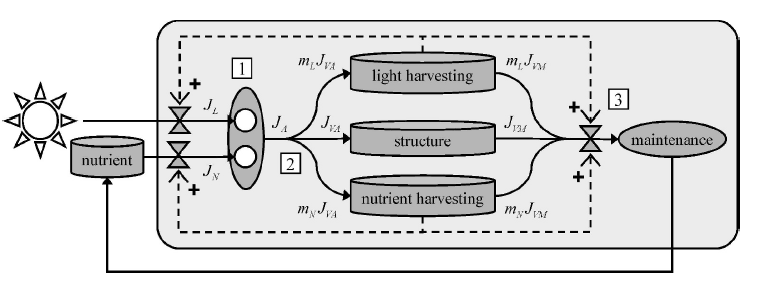
\includegraphics[trim = 0mm 0mm 0mm 0mm, clip, width=1\linewidth]{./Chp3-Further/Bruggeman-2007.png}
\caption[Scheme]{\small {Bruggeman and Kooijman model scheme. Taken from \citet{Bruggeman2007}}}
\label{Bruggeman}
\end{figure}

In 2007 \citet{Bruggeman2007} developed a trait model based on DEB concepts to study phytoplankton diversity and succession. The model (\ref{Bruggeman}) captures the seasonal dynamics of the phytoplankton community structure and key process which influence diversity, such as migration. However, they had to face the problem of having to consider too many species (and therefore too many state variables and parameters) when tackling biodiversity studies. \citet{Bruggeman2007}, however, elegantly resolved the problem by approximating the full model with a simpler one. Using a moment closure technique to estimate the few, most important macroscopic properties of the full, complex system, such as total biomass, mean trait value, and trait variance, as previously proposed by \citet{Wirtz1996, Norberg2001}, Bruggeman and Kooijman's(\citeyear{Bruggeman2007}) obtained a simpler model, which dynamics compared remarkably well with the one of the full model. It should be noted, however, that this method assumes a normal distribution of the trait possibly omitting interesting multimodal dynamics \citep{Bruggeman2007}. Following studies refined this approach by providing a complete mechanistic framework for developing these kind of models and by confirming the quality of the approximation in capturing the essential physiological and ecological characteristics of the full model \citep{Merico2009}. 

\subsection{Method}
The main focus of my PhD work is to develop a size-based model following the approaches of  \citet{Bruggeman2007, Merico2009} in order to further explore the detailed mechanisms leading to the observed phytoplankton size structure distributions in regions of the Atlantic Ocean of contrasting environmental conditions. The guiding principle for defining the traits and the tradeoffs to be incorporated into my model will be based on the concept that organisms face trade-offs in their ability to allocate limited energy and resources to growth, reproduction and defence, which is central to most theories explaining the diversity of life on Earth \citep{Tilman2000}. Based on available observations, I will therefore develop a trade-off between competitive ability for nutrient acquisition and resistance to grazing (\ref{model}). I will then include a specific grazing pressure that relates to both phyto- and zooplankton mortalities.

The resulting, full size-based model will be approximated with a simpler model of aggregate macroscopic properties using the moment closure approximation proposed by \citet{Wirtz1996, Norberg2001} and further refined by \citet{Bruggeman2007, Merico2009}. The phytoplankton total biomass ($P$), the mean trait ($\bar{s}$), and the trait variance ($v$) will be formulated as follows:

\begin{align*}
\frac{dP}{dt} & = \left[r(\bar{s})+\frac{1}{2}v\frac{\partial^{2} r(\bar{s})}{\partial s^{2}}\right]P \nonumber \\
& \nonumber \\
\frac{d\bar{s}}{dt} & = v\frac{\partial r(\bar{s})}{\partial s}\nonumber \\
&\nonumber \\
\frac{dv}{dt} & = v^{2}\frac{\partial^{2} r(\bar{s})}{\partial s^{2}}\nonumber\\
\end{align*}

The approach of defining a trade-off that relates size to the competitive ability for nutrient acquisition and resistance to predation \citep{Merico2009} leads to mechanistically capture bottom-up (nutrient availability and acquisition capabilities) versus top-down (avoid grazing) processes, major shaping forces of a phytoplankton community. The model will be tested against and constrained by the AMT observations on environmental data and community size structures in the Atlantic Ocean (chapter 2).  

\begin{figure}
\centering
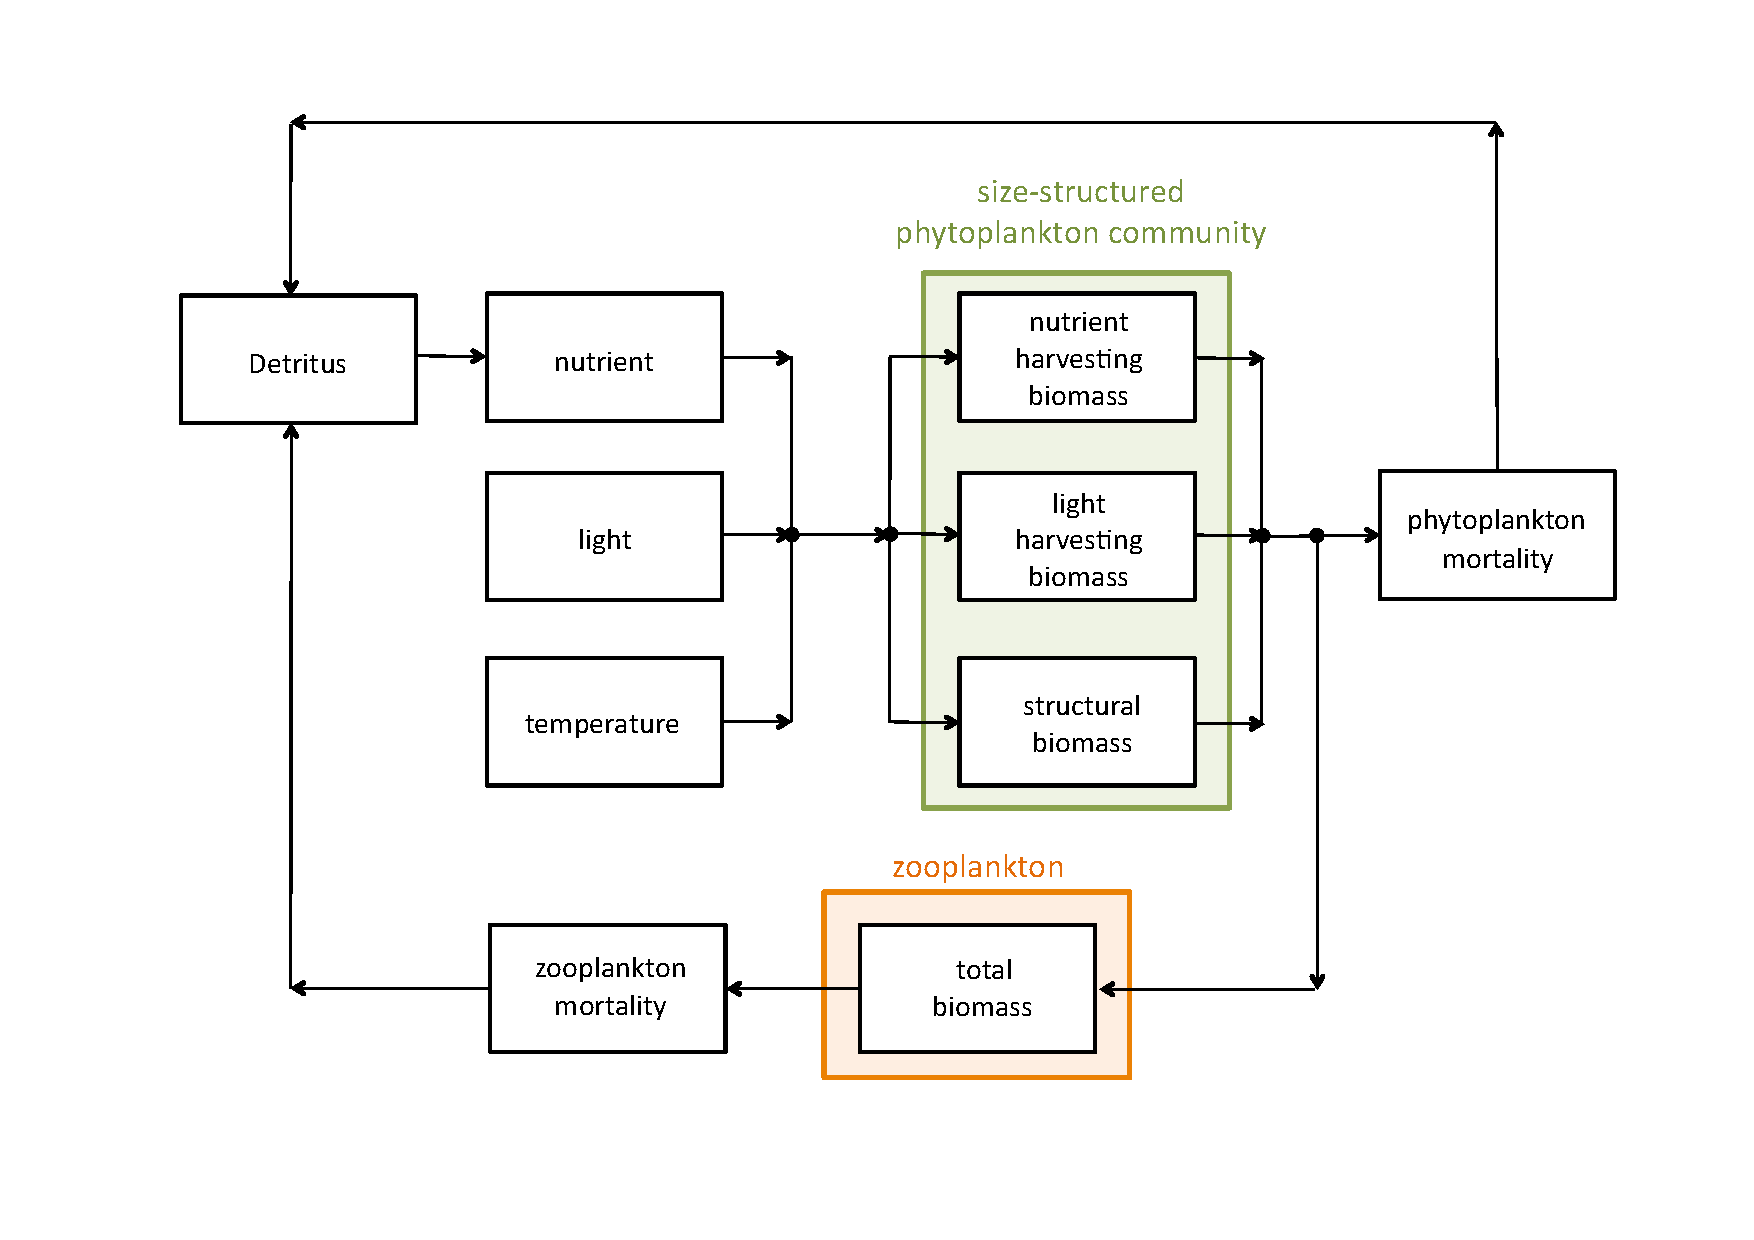
\includegraphics[trim = 15mm 50mm 15mm 25mm, clip, width=1\linewidth]{./Chp3-Further/model-scheme.pdf}
\caption[Scheme]{\small {Scheme of the proposed size-based model. In this model phytoplankton allocates energy (or biomass) to different pools such as nutrient and light harvesting biomasses and generic structural biomass. A certain fraction of the phytoplankton biomass flows into the zooplankton biomass and a remaining fraction is remineralized into the nutrient pool}}
\label{model}
\end{figure}

\subsection{Relevance}
The work proposed with this PhD project will be important for further developing trait-based models of planktonic communities. Previous studies have not been able to consistently address complex adaptive systems with a reduced amount of complexity. The ability to model a complex system as a single adaptive entity while retaining the most fundamental ecological processes shaping its dynamics is doubtlessly elegant and attractive. 

As shown in chapter 2, different regions in the Atlantic Ocean have specific community patterns. With my model I will attempt to capture the observed community structures regions of the Atlantic Ocean with contrasting environmental conditions. To our knowledge no effort have been made yet to develop such a trait-based model in this region of the world. As typical of any modelling study, my work will provide also quantitative understanding of the relative contribution of the most important physiological and ecological processes shaping the phytoplankton community size structure. 

A key aspect with our approach is that under any given environmental condition, typical community size-structures will emerge consistently to the Bass Becking's principle that "Everything is everywhere, but the environment selects" \citep{BaasBecking1934}. More generally, I expect that this work will provide the possibility to test different ecological hypothesis proposed for explaining biodiversity, including the niche and the neutral hypotheses \citep{Hubbell2001,Mcgill2003}.

\section{Multi-trait size-based model}
A recent review on the current developments of plankton models by \citet{Follows2011} stress that most of the trait-based models elaborated so far have been only focusing on photoautotroph. It appears reasonable to start extend trait-based formulations also to other groups such as zooplankton, as in our proposed size-based model (\ref{model}). I will therefore extend my model to include a dynamic selection of the prey based on the size of predator.

I believe that the allometric scaling of predator-prey interactions in planktonic systems is a key aspect for further advances in trait-based models due to the importance of this process in regulating the phytoplankton community structure\citep{Agrawal2001, Litchman2008}. Technically, I will mechanistically derive two trade-off functions, one for the phytoplankton as explained in the previous section, and the other for the zooplankton. The new trade-off function will be based on the size of the zooplankton and on the size of the predated phytoplankton. The type of model approximation used will be the once estimated from the moment closure, in analogy to the size-based model proposed in section 3.1.2.

With this multi-trait implementation we expect to reduce the parameterization and overall complexity of early models possibly leading to a significant advance in plankton ecosystems modeling by developing a more parsimonious mechanistic description.

\section{Paleo-reconstruction of planktonic communities}

\begin{figure}
\centering
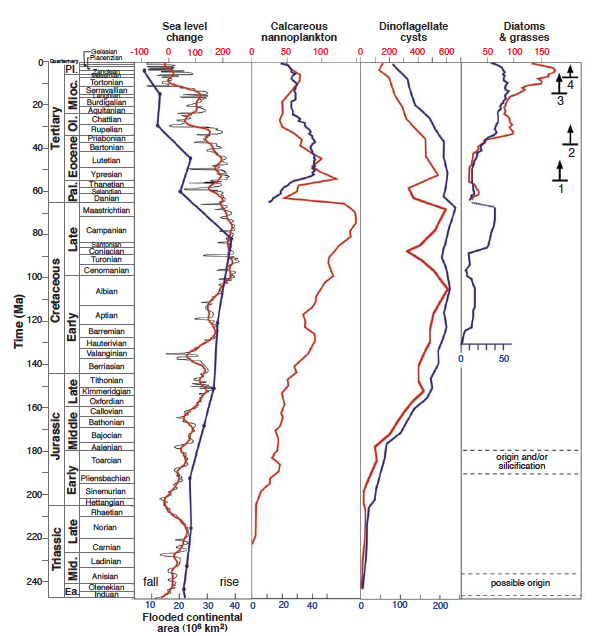
\includegraphics[trim = 0mm 0mm 0mm 0mm, clip, width=1\linewidth]{./Chp3-Further/Falkowski-2004.png}
\caption[Scheme]{\small {Comparison of major phytoplankton groups with sea-level change. The red line accounts for species diversities from published studies. The blue line accounts for the genus diversity compiled from public databases by the authors. Taken from \citet{Falkowski2004a}. }}
\label{Falkowski}
\end{figure}

Since Darwin times, ecologist have tried to understand the evolutionary processes that lead to the current patterns of biodiversity. \citet{Hutchinson1961} was fascinated by the capacity of phytoplankton communities to produce such  a large diversity from a limited range of resources fro which they compete. In the history of life on Earth, phytoplankton emerged at around 2.5 billion years ago when cyanobacteria started to spread in the earth oceans, thus creating an enormous impact on the global environment. Later $\sim$ 1.6-1.8 billion years ago, unicelular eukaryotes raised when they started to "use" prokaryotic cells as their metabolic slaves. From that point on, different kind of unicellular eukaryotes emerged, until three characteristic groups of phytoplankters originated from an ancestral red alga, and started to dominate earths aquatic environments (Figure \ref{Falkowski}) \citep{Falkowski2004a}. Since the Middle Triassic these well know groups, dinoflagellates, coccolithophores and diatoms, began to play an important role on the biogeochemistry of our planet and supported a wide range of life forms in more and more complex food webs \citep{Falkowski1998}.

\citet{Jiang2005,Litchman2009} develop a size-based evolutionary model, based on game theory, to determine the driving processes which could produce  the difference size distributions of diatoms. Their model results suggest the nitrogen to phosporus stoichiometric ratio, the nutrient fluctuation, and the changes on mixed layer depth, as major mechanisms leading the size differences in diatoms. 

Following these approaches, I plan to adopt my trait-based modelling approach to study the changes in the phytoplankton community composition during the Cenozoic period. This approach will be based on the size-based model developed for the Atlantic Ocean but obviously appropriately set up for targeting environmental changes operating on a geological time scale. The species diversity will be mechanistically captured in my model  by the variance of the trait distribution, and the prevaling mean trait value at a specific time will give an indication of the characteristic group or species dominating the community. Due to the distinct morphological differences in the three functional groups, it is appropriate to use size as a key trait to disentangle the different mechanisms shaping phytoplankton diversity across the Cenozoic era. 

\newpage

\section{Time table} 

\begin{figure}[h]
\centering
\includegraphics[trim = 20mm 25mm 20mm 25mm, clip, width=1\linewidth]{./Chp3-Further/Chronogram.pdf}
\end{figure}

